\documentclass[10pt, titlepage, oneside, a4paper]{article}
\usepackage[style=numeric]{biblatex}
\addbibresource{bibliography.bib}

\usepackage[T1]{fontenc}
\usepackage[titletoc]{appendix}
\usepackage[utf8]{inputenc}
\usepackage{amssymb, graphicx, fancyhdr}
\usepackage{amsmath}
\usepackage{amsthm,algorithm,algorithmic,yhmath,enumitem,lscape}
\usepackage{float}
\usepackage{hyperref, url}
\usepackage{minted}
\newmintinline{c}{}
\addtolength{\textheight}{20mm}
\addtolength{\voffset}{-5mm}
\def\inst{Computing Science}
\def\course{5DV243 Artificial Intelligence}
\def\title{Assignment 1 --- Othello}

%%%%%%%%%%%%%%%%%%%%%%%%%%%
\def\names{Sienichev Matvey, Afrasah Benjamin Arko} 
\def\csusernames{ens25msv, mai25bah}
\def\graders{Filip Naudot, Timotheus Kampik, Igor Ryazanov}
%%%%%%%%%%%%%%%%%%%%%%%%%%%%


\def\mfullpath{\raisebox{1pt}{$\scriptstyle \sim$}\musername/\path}
\def\nfullpath{\raisebox{1pt}{$\scriptstyle \sim$}\nusername/\path}
\newcommand{\R}{\mathbb{R}}
\newcommand{\N}{\mathbb{N}}
\newcommand{\Rnn}{\mathbb{R}^{n \times n}}
\newcommand{\bes}{\begin{equation*}}
\newcommand{\ees}{\end{equation*}}
\newcommand{\be}{\begin{equation}}
\newcommand{\ee}{\end{equation}}
\newcommand{\bms}{\begin{multline*}}
\newcommand{\emults}{\end{multline*}}
\newcommand{\bbm}{\begin{bmatrix}}
\newcommand{\ebm}{\end{bmatrix}}
\newcommand{\eps}{\epsilon}
\newcommand{\fl}{\text{fl}}
\newcommand{\Lp}{{L^p}}
\newcommand{\Ker}{\text{Ker}\,}
\newcommand{\loc}{{\text{loc}}}
\newcommand{\ccinf}{C_c^\infty}
\newcommand{\supp}{\text{supp}}
\newcommand{\dist}{\text{dist}}

\begin{document}
	\begin{titlepage}
		\thispagestyle{empty}
		\begin{large}
			\begin{tabular}{@{}p{\textwidth}@{}}
				\textbf{\hfill \today} \\
				
				%\textbf{\typeofdoc} \\
			\end{tabular}
		\end{large}
		\vspace{25mm}
		\begin{center}
			%\LARGE{\pretitle} \\
			\huge{\textbf{\course}}\\
			\vspace{10mm}
			\LARGE{\title} \\
			\vspace{15mm}
            \LARGE{version 1.0} \\
            \vspace{10mm}
			\begin{large}
				\begin{tabular}{ll}
					\textbf{Names} & \names \\
					\textbf{CS usernames} & \csusernames 
				\end{tabular}
			\end{large}
			\vfill
            \vfill
			\large{\textbf{Graders}}\\
			\mbox{\large{\graders}}
		\end{center}
	\end{titlepage}
    
    % fixar sidfot
	%\lfoot{\footnotesize{\name, \username}}
	\rfoot{\footnotesize{\today}}
	\lhead{\sc\footnotesize\title}
	\rhead{\nouppercase{\sc\footnotesize\leftmark}}
	\pagestyle{fancy}
	\renewcommand{\headrulewidth}{0.2pt}
	\renewcommand{\footrulewidth}{0.2pt}

	% skapar innehållsförteckning.
	% Tänk på att köra latex 2ggr för att uppdatera allt
	%\pagenumbering{roman}
	%\tableofcontents
	% och lägger in en sidbrytning
	%\newpage

	\pagenumbering{arabic}

	% i Sverige har vi normalt inget indrag vid nytt stycke
	\setlength{\parindent}{0pt}
	% men däremot lite mellanrum
	\setlength{\parskip}{10pt}

\addtocounter{section}{0}
%\section{Changes}
%If this is a resubmission, include a list of changes %with respect to
%the previous submission.

\section{Introduction}
\label{sec:intro}
% Also possible to use \input{intro.tex} to break down the report into one file per section
Robots have been beating humans in more and more domains every day. This is also the case for Othello, a strategic turn based board game. As such to fight fire with fire, we attempted to create an Othello game engine capable of outperforming a simple fixed depth search of 7, piece count based game engine. 
We used python for this task, which can be around 10 to 100 times slower than a compiled language, because of that we had to use a couple of tricks to outcompete a Java written engine withing reasonable compute times, ideally in less than 3 second per move, both as black and as white player. To achieve these times while still keeping a sufficient compute depth our engine implements alpha beta search algorithm that offers a substantial speed up compared to a min/max algorithm. While that that allows us to go to depths grater than 7 in the early game, as well as in the endgame, during midgame the branching factor is too high to allow it to compute in under 3 seconds, that's why our algorithms uses an iterative deepening approach, starting at depth 3 and evaluating iteratively deeper and deeper as long as the maximum time for the move hasn't been exceeded. Unfortunately, that means that for some moves the decisions are made having less information about all the possible states of the board than the adversary. To make up for the short-sightedness of our algorithm we implemented some clever heuristics that mimic human long term strategy thinking to evaluate the score of every position. 
Firstly we will discuss the technical details of our implementation\ref{sec:methods}, after than we will give results \ref{sec:results} and finally analyze them and discuss possible improvements \ref{sec:discussion}



\subsection{Reproducibility and Environment}
State your language (Java or Python), version, compiler/interpreter flags, and OS.
Include how to run your engine with the provided \texttt{othello.sh}:
\begin{minted}{bash}
./othello.sh <position_string> <time_limit_seconds> <do_compile>
# Example:
./othello.sh WEEEE... 5 0
\end{minted}

\section{Methods}
\label{sec:methods}


\subsection{Position Representation}
Currently a position is being stored as an array of arrays 10 by 10 of 8 bit characters, with the borders being empty, so effectively only a 64 square zone is used to play. 
Every square in othello game can be either occupied by a black disk, a white disk or empty. These 3 states are represented by storing a 'W', a 'B' or an 'E' characters in the array representing the board.
For example to put a white disk on a first row of a second column, we do it as shown in Figure~\ref{fig:board_representation}
\begin{figure}[h]
    \centering
    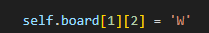
\includegraphics[width=0.6\textwidth]{img/board_representation}
    \caption{Board representation}
    \label{fig:board_representation}
\end{figure}
This is the easiest way to do it because it is an straight forward implementation of a real world othello board as we humans perceive it. 



 bitboards), how you compute legal moves, how you apply a move (including flipping discs), and how you detect terminal states and scoring.
If you adopted the provided helper code, mention which parts you completed (the \texttt{TODO}s) and any optimizations you added.

\subsection{Search Algorithm: Alpha--Beta}
Describe your Alpha--Beta implementation: function signature, maximizing/minimizing roles (white = MAX, black = MIN),
cutoff conditions (depth/terminal), and how you propagate values.
If you used enhancements (move ordering, transposition table, aspiration windows), explain them concisely.

\subsection{Iterative Deepening \& Time Control}
Unlike the naive player which searches at a fixed depth of 7, we implemented 
\textit{Iterative Deepening Search (IDS)} with depth increments of 1. 
This gives us the best move from the deepest search we managed to complete 
until we ran out of time.

Our time control is cooperative. We check the clock during a search and throw 
a \texttt{StopSignal} exception when time runs out. The exception is caught by 
the main loop and returns the best move so far. For each iteration, we compute 
the remaining time and pass it to our \texttt{AlphaBeta} algorithm, which checks 
at every 1000th node if we have enough time.

In order not to run out of time, we utilize 90\% of the allocated time. 
This gives us a small buffer for evaluation overhead while maximizing our 
search depth.

One main advantage of iterative deepening is that even if we get cut off 
mid-search, we still have a complete result from previous depths.

% Explain how you replaced fixed-depth with Iterative Deepening Search (IDS) and describe how you enforce your time budget. 

% If your search is \emph{cooperative}, describe where you check time (e.g., on node entry, inside move loops), how you signal timeout (e.g. return flag or exception), and how the top-level search preserves the best move from the last completed depth.

% Optionally discuss thread/process-based control (e.g., main thread owns the clock; worker thread does search and checks a stop flag).
% If you used a hard cutoff (separate process), briefly explain the serialization of moves.

\subsection{Heuristics}

For our heuristics, our evaluation function is a significant development of the \texttt{CountingEvaluator} which just counts pieces. We developed a 10 feature heuristic system that captures the strategic features of Othello gameplay through careful analysis of established game theory and empirical testing.

\subsubsection{Evolution from CountingEvaluator}
The \texttt{CountingEvaluator} gave a basic evaluation by just counting the difference between the discs of the current player and the opponent:
\begin{equation}
\text{Score} = \text{my\_pieces} - \text{opp\_pieces}
\end{equation}

This approach only has merit in the last phase of the game when mobility is limited and does not capture the strategic complexity of Othello. Our enhanced evaluation addresses the limitations of piece counting through a comprehensive analysis of features that affect gameplay.

\subsubsection{Feature Engineering and Strategic Analysis}

Our evaluation uses a weighted linear combination with 10 strategic features:
\begin{equation}
\text{Score} = \sum_{i=1}^{10} w_i \cdot f_i
\end{equation}
Where $w_i$ are the optimized weights and $f_i$ are the extracted features. The features are calculated from the perspective of the starting player.

We improved our weights by focusing on stability, mobility and corner control, and penalizing dangerous positions through gameplay analysis and testing with the naive\cite{brianothello2005}.
Overall, we managed to capture the limitations of the naive piece counting player.

\begin{table}[H]
\centering
\footnotesize
\begin{tabular}{|l|l|c|c|}
\hline
\textbf{Feature} & \textbf{Formula} & \textbf{Weight} & \textbf{Description} \\
\hline
\multicolumn{4}{|c|}{\textbf{Stability Control}} \\
\hline
Corner Control & $my\_corners - opp\_corners$ & 600.0 & Corner occupation \\
\hline
Edge Control & $my\_edges - opp\_edges$ & 70.0 & Edge position control \\
\hline
Stability & $my\_stability - opp\_stability$ & 90.0 & Unflippable discs \\
\hline
\multicolumn{4}{|c|}{\textbf{Risk Avoidance}} \\
\hline
X-Squares & $my\_x\_squares - opp\_x\_squares$ & -50.0 & Dangerous corner-adjacent \\
\hline
C-Squares & $my\_c\_squares - opp\_c\_squares$ & -5.0 & Risky corner-adjacent \\
\hline
Frontier Discs & $my\_frontier - opp\_frontier$ & -10.0 & Vulnerable flippable pieces \\
\hline
\multicolumn{4}{|c|}{\textbf{Mobility Control}} \\
\hline
Mobility & $my\_mobility - opp\_mobility$ & 100.0 & Legal moves available \\
\hline
Potential Mobility & $my\_potential - opp\_potential$ & 6.0 & Future move opportunities \\
\hline
\multicolumn{4}{|c|}{\textbf{Piece Difference}} \\
\hline
Piece Difference & $my\_pieces - opp\_pieces$ & 100.0 & Disc count advantage \\
\hline
\multicolumn{4}{|c|}{\textbf{Game Phase Adaptation}} \\
\hline
Parity Score & 1 or 0 & 18.0 & Move timing control \\
\hline
\end{tabular}
\caption{Complete Heuristic Feature Set with Formulas and Weights}
\end{table}


\setcounter{secnumdepth}{4}
\subsubsection{Stability Control}

\vspace{0.5em}

\textbf{Corners} (Weight: 600.0) are the most strategically important positions because they can never be flipped once captured\cite{brianothello2005}.  They serve as a foundation for building more stable discs. They make it possible to build more stable discs and often decide the outcome of the game\cite{brianothello2005}.

\textbf{Edge positions} (Weight: 70) gives strategic advantages for making paths to corners and making it harder for your opponent to move.  But they need to be balanced carefully, because taking the edge too soon can make you weak in the early game\cite{brianothello2005}.  The medium weight shows how important edge control is, which gets more important as the game goes on.

\textbf{Stable discs} (Weight: 90.0) are those that no opponent move can flip.  Our stability analysis uses a simple heuristic method to estimate stability, taking into account the following: (1) corners are always stable and worth 3x as much, (2) edges are somewhat stable and worth 1x as much, and (3) interior pieces are assumed to be neutral and not counted.  This method of estimating disc stability gives a good idea of how stable it is without the need for complicated calculations \cite{othello-heuristics-analysis}. 



\subsubsection{Risk Avoidance}

\vspace{0.5em}

\textbf{X-Squares} (Weight: -50.0) are the diagonal squares next to the corners.  These positions are very risky because they often let the other player capture the corner \cite{brianothello2005}.  The strong negative weight shows that the tactical rule is to avoid X-square occupation unless it is absolutely necessary.

\textbf{C-Squares} (Weight: -5.0) are squares that are right next to corners.  C-squares are less dangerous than X-squares, but they can also lead to corner loss through tactical sequences \cite{brianothello2005}.  
The moderate negative weight reflects how occupying a C-square might be okay in some situations.

\textbf{Frontier Discs} (Weight: -10.0) are those next to empty squares. We negatively weight them because having more frontiers reduces your stability and increases your opponent's mobility\cite{brianothello2005}.

\subsubsection{Mobility Control}

\vspace{0.5em}

\textbf{Mobility} (Weight: 100.0) is the number of legal moves a player can make.  High mobility gives players the freedom to make strategic and tactical choices, which lets them avoid being forced to move to bad positions \cite{cohen2020learning}.

\textbf{Potential Mobility} (Weight: 6.0) counts empty squares next to opponent pieces, which show where they could move in the future.  A higher opponent potential mobility is bad because it means they have more strategic options\cite{buro1995othello}.  This feature helps you think about long-term tactical options that go beyond just legal moves right now.

\subsubsection{Piece Difference}

\vspace{0.5em}

\textbf{Piece Difference} (Weight: 100) plays a significant role in the last stages of the game when mobility is limited \cite{othello-heuristics-analysis}.

\subsubsection{Game Phase Adaptation}

\vspace{0.5em}
\textbf{Parity Score} (Weight: 18.0) determines tempo advantages based on remaining moves and current disc count. If remaining moves are even, the player ahead in discs has advantage. If remaining moves are odd, the player behind in discs benefits from the extra move \cite{brianothello2005}. This binary feature (0 or 1) helps evaluate endgame positioning and move timing advantages.

\subsection{makeMove() / Action Generation}
Describe your move-generation procedure and any invariants. Explain how you handle pass moves.

\section{Results}
\label{sec:results}
Explain your test methodology: opponents (naive engine), time limits (2--10~s), colors (white and black), and the metrics you report (win/loss, disc difference, depth reached, nodes visited if available).
Mention any randomness and how you controlled it.


\subsection{Test runs}
\label{sec:testruns}
Present your main results table (example in Table \ref{tab:othello-results}) and describe them in text (what trends do you observe? where do you gain the most?).

COUNTING EVALUATOR

\begin{table}[h]
    \centering
    \caption{Performance as White and Black using a counting evaluator}
    \begin{tabular}{cccc}
    \hline
    \textbf{Color} & \textbf{Time limit} & \textbf{Result}&\textbf{ average depth} \\
    \hline
    White & 3s & XX won with YY & 5\\ 
    Black & 3s &  &\\
    White & 5s &  &\\
    Black & 5s &  &\\
    White & 8s &  &\\
    Black & 8s &  &\\
    \hline
    \end{tabular}    
    \label{tab:othello-results}
\end{table}

HEURISTIC:

\begin{table}[h]
    \centering
    \caption{Performance as White and Black using a position evaluation heuristic}
    \begin{tabular}{cccc}
    \hline
    \textbf{Color} & \textbf{Time limit} & \textbf{Result}&\textbf{ average depth} \\
    \hline
    White & 3s & XX won with YY & 5\\ 
    Black & 3s &  &\\
    White & 5s &  &\\
    Black & 5s &  &\\
    White & 8s &  &\\
    Black & 8s &  &\\
    \hline
    \end{tabular}    
    \label{tab:othello-results}
\end{table}

\section{Discussion}
\label{sec:discussion}
Representing the boart as an array of array is easy to implement, howerver, it is not very efficient. Indeed, each character takes 1 byte of memory, so a full board takes 100 bytes. 

MEMORY IMPROUVEMENTS:


The deeper we go, the more positions we have to evaluate, for example for the depth of 7 with a random evaluation ordering, we can on average achieve a compelxity of $O\big(b^{3d/4}\big)$ \textcite{alpha_beta_complexity} so with a branching factor of 10 the number of positions to evaluate would be 177 830, taking 100 bytes per position, the memory usage would be around 16 Megabytes, wich is not that much and can fit in a cache of a modern cpu, however the using the same calculation for a depth of 10 would yeild 31 millions positions to evaluate and would take 3Gb in memory alone, that whould not fit in a cache of any cpu, so frequents memory swaps will slow it down. However, python class instance is memory intensive in itself so => data structure = insignifican in comparaison => should have wrotten it in C(not class language)

=>bitboard = 2*64 bits => 2bytes
31 millons position => 62 million bytes => only 59mb => couple mem swaps


COMPUTE IMPROUVEMENTS:





\textbf{Interpret the results. Explain why your heuristic and move ordering helped (or where they fell short).}
\textbf{Discuss failure cases, time overruns (if any), and the trade-off between deeper search and evaluation quality.
Relate back to the assignment requirement: did you consistently beat the naive engine under 2--10 s as both colors?}


\section{Reflections}
\label{sec:reflections}
Briefly describe your development process, challenges, and lessons learned (e.g., debugging move generation, off-by-one errors in indices, ensuring legal flips, enforcing time limits robustly).

Outline how you divided work and ensured both partners understood the entire solution.
\textcite{brianothello2005}
\textcite{buro1995othello}
\textcite{jaskowski2014ntuple}

\printbibliography










\subsection{Source code}
\label{app:source-code}
If you wish to include any source code in this report, you may use the
\emph{minted} or \emph{listings} packages. The example below shows \emph{minted}.

\begin{minted}[linenos=true=autogobble]{c}
/* Example main */
int main(void) {
    return 0;
}
\end{minted}
\end{document}